\documentclass[12pt]{report}

\usepackage[left=1in, right=1in]{geometry}
\usepackage{fancyhdr}
\pagestyle{fancy}


\usepackage{graphicx}
\usepackage{enumitem}
\usepackage{geometry}

\usepackage{listings}
\lstset{language=Java, numbers=left}
\usepackage[usenames, dvipsnames]{color}

\usepackage{array}							% apply style to column

\definecolor{codegray}{gray}{0.9}
\newcommand{\code}[1]{\colorbox{codegray}{\texttt{#1}}}


\usepackage{url}

\usepackage{setspace}
\doublespacing

\usepackage{titlesec}
\titleformat{\chapter}
    {\large\bfseries} % format
    {}                % label
    {0pt}             % sep
    {\huge}


\fancyhf{}
\fancyhead[RE]{\leftmark}
\fancyhead[LO]{\rightmark}
\fancyhead[LE,RO]{\thepage}
\renewcommand\headrulewidth{0pt}
\renewcommand\chaptermark[1]{\markboth{#1}{}} 
\renewcommand\sectionmark[1]{\markright{\thesection.\ #1}}

\setcounter{secnumdepth}{3}
\setcounter{tocdepth}{3}

\usepackage[nottoc]{tocbibind}
\renewcommand{\bibname}{References}

\begin{document}

    \begin{titlepage}
	\centering
	
	%\vspace{-5.0cm}
	
    
\includegraphics[width=0.7\textwidth]{images/wpiLogo.png}\par\vspace{0.0cm}
	
    {\scshape\Large Worcester Polytechnic Institute \par}
	\vspace{0.5cm}
	
    {\scshape\large
		A Major Qualifying Project submitted to the Faculty of the 
		Worcester Polytechnic Institute in partial fulfillment of 
		the requirements for the Degree of Bachelor of Science on April 27, 2016 
	\par}
	\vspace{0.5cm}
	
    {\LARGE\bfseries Data  MATTERS: Customizing Economic Indices to Measure State Competitiveness \par}
	\vspace{1cm}
	
    {\large\itshape 
        Bogatov, Dmytro \texttt{dbogatov@wpi.edu} \\
        Hennessy, Jillian \texttt{jrhennessy@wpi.edu}
     \par}
	\vfill
	
    supervised by\par
	Professor Elke Rudensteiner

	\vfill
    
\end{titlepage}

    \chapter*{Abstract}
	
The goal of this project was to expand the functionality of the Massachusetts 
Technology, Talent, and Economic Reporting System (MATTERS) for the 
Massachusetts High Technology Council (MHTC), a protechnology advocacy and 
lobbyist organization, with two new features - Application Program Interface
(API) and Metric Builder. API defines a communication protocol between MATTERS 
and other computational-based systems. We also wrote an extensive API 
documentation. Metric Builder is a tool that lets users create own metrics with
own rules out of existing MATTERS metrics. Users are now able to define their
own indexes and track individual states' performance.

    \pagebreak

    \chapter*{Executive Summary}
\addcontentsline{toc}{chapter}{Executive Summary}

Data is a large part of every industry in the business world and big data can help create value in these industries by providing various analytics and performance measures that were once not readily available. Gathering and analyzing this data can drive growth and lead to better decision making across industries. The Massachusetts High Technology Council (MHTC) actively works to maintain Massachusetts' reputation as a competitive business environment in technology based sectors. With this in mind, MHTC worked to create MATTERS, the Massachusetts Technology, Talent, and Economic Reporting System, which is a web dashboard designed that allows users to access and visualize data collected from a large number of other sites. MATTERS allows users to compare economic, educational, demographic and other aspects across states.
 
The goal of our project was to introduce two new features to MATTERS that would allow for users to interact with the collected data in more ways than previously available. The ability to display and analyze data in new ways would help to continue MHTC's goal of showing Massachusetts as a competitive state for businesses that are high tech. To achieve this goal we completed the following:
\begin{itemize}
 	\item Create the Metric Builder to allow MHTC along with other registered users to create their own metric formula using the preexisting metrics stored in MATTERS
 	
 	\item Create a public facing API and corresponding documentation for the site to allow developers a system-friendly way to access the data that MATTERS stores
 	
 	\item Test the features to ensure that they are easy to use for both technical and non-technical users
 \end{itemize} 
 
Before the creation of the Metric Builder page, users could compare states and years by looking at the preexisting metrics found in the MATTERS database. This limited the way users could innteract with the data. MHTC wanted a way to store their own custom metrics which led to the creation of the Metric Builder page. Using the Metric Builder, users now have the ability to choose any number of metrics and assign different weights to indicate how important each metric was compared to the others selected. The Metric Builder feature would build the custom metric formula for the users and normalize the data values, allowing users to visualize their custom metrics consistently just as they would any metric in the site already. As a result of the creation of the Metric Builder, MHTC used our metric formula tool to create four custom metrics that will be displayed on the home page of the MATTERS site.
 
Meanwhile, the creation of the API helped to provide developers with a means of extracting desired data values in a system friendly way. Previous to implementing a public facing API, the only way to access the raw data would be through parsing the HTML. Having an API for the site makes the data more widely available to the public and helps developers save time and reduce errors by not having to scrap MATTERS for data. During this implementation two things needed to be considered; a way to have users access all of the data securely and how developers would know how to send proper API requests. To make sure the data was accessed securely, a common practice which we adopted was the creation of an API key. Users will receive a specific API key identifier and this will give them access to the data while also allowing us to keep track of who is accessing the data values at any time. To make the API easy to use, API documentation was created following standard practices of API documentation for sites.
 
With these new features now in place, users will be able to interact with the available data in even more ways than previously available from both the user side and the system side. This will continue to make MATTERS a useful tool for both MHTC and other users, and continue to aid MHTC's goal to make Massachusetts a competitive environment for high-tech businesses.
 
Upon completion of this project, we have developed a set of recommendations for those who will continue to work on MATTERS in the future. The recommendations are as follows:
 
 	\begin{itemize}
 		\item MATTERS system
 		\begin{enumerate}
 			\item
 			Let users define more complex equations for their user metrics.
 			User should not be limited by simple weighted average formula.
 			\item
 			Let users suggest corrections to data or even new data sources. Right now 
 			MATTERS' administrators and data management team are working on
 			adding data. By involving users in this process, MATTERS may have 
 			more complete, accurate and up-to-date data.
 			\item
 			Role management. Right now the system supports regular users and API users. 
 			Each user metric must have one and only one author. It might be a good idea 
 			to merge these two user entities and introduce shared user metrics that are 
 			not bound to specific users.
 		\end{enumerate}
 		\item Software development
 		\begin{enumerate}
 			\item
 			Refactor the client side and server side code. Since the system 
 			has been developed by a number of teams with different design 
 			patterns and approaches, there is a significant technical debt. 
 			It might be worth spending some time rewriting parts of the system 
 			according to the latest coding and technical standards.
 			\item
 			Documentation. Right now there is a steep learning curve for new 
 			developers who start working on the project. Good documentation would decrease the time it takes for developers to start working 
 			on the project.
 		\end{enumerate}
 	\end{itemize}
    \pagebreak

    \chapter*{Acknowledgements}
	
We would like to thank and acknowledge the following for all their help, support, and contributions to this project:
\begin{itemize}
	\item Massachusetts High Technology Council for making this project possible and working with Worcester Polytechnic Institute to create and grow MATTERS
	
	\item Professor Elke Rundensteiner from WPI for her assistance and guidance throughout the entire project
	
	\item Caitlin Kuhlman from WPI for her help throughout the project and providing guidance and feedback on all aspects of the project
	
	\item Worcester Polytechnic Institute for allowing us the opportunity to work on this MQP project 
\end{itemize}
    \pagebreak

    \tableofcontents
	
	\listoffigures
	\listoftables
	

    \chapter{Introduction}

	With the total amount of data in the world growing steadily at a fast rate, 
	the need to analyze large amounts of data in datasets, also called big data, is a 
	key driver for productivity growth and innovation [10]. With this increase in 
	information often freely available across the web, 
	the Internet will continue to provide a basis for the continued growth of 
	data in the future. Data is a part of every industry and business in today's 
	world from retail to government. Big data and can help to create
	 value in these industries by making information more usable, showing more 
	 accurate performance measures, and providing detailed analytics on this data that 
	 leads to better decision making.

	In this data-driven time, it is important to be able to make decisions 
	quickly using the data that is available. Big data visualization is an 
	effective way to present the important information amongst the large amount 
	of data used and helps to drive complex analysis \cite{bigdata}. Big 
	data analysis, it can make otherwise too large amounts of data meaningful 
	to those who looking to interpret significance from it.

	The Massachusetts High Technology Council, or MHTC \cite{mhtc}, is a group of technological, 
	professional and higher education executives across the state of Massachusetts. 
	They are comprised of higher education CEOs, senior executives from Massachusetts 
	and more. For over thirty-eight years, MHTC has advocated for policies 
	and programs to create and keep both a healthy and competitive business climate in Massachusetts. 
	Their goal is to establish and keep Massachusetts as a competitive place for 
	successful business and talent building, including in particular with a specific focus on the 
	technology sectors. In part because of the MHTC and its members, who are 
	regarded as the region's most venerable technology association, Massachusetts 
	is regarded as one of the top competitive areas for businesses that are “high tech” \cite{mhtc}.

	The Massachusetts Technology, Talent, and Economic Reporting System,also known as MATTERS, 
	was developed by MHTC along with Worcester Polytechnic Institute (WPI) and other 
	institutions as a collaborative effort designed to aid users in understanding a 
	variety of public data in an effort to help make Massachusetts the top location 
	for high technology businesses. MATTERS uses this data collected to both measure 
	and evaluate the current state of Massachusetts compared to other states in the 
	country. It provides policy makers and advocates with easily accessible and search-able 
	dynamic data to assist in their efforts regarding decisions to help  retain and 
	grow business in the state. MATTERS integrates a wide 
	range of talent, cost, and economic metrics and state rankings from federal and 
	state government sources, non-profit organizations and media outlets into one 
	location via a data warehouse for its users \cite{about}. 

	Previously to our project, WPI IQP, MQP and graduate student teams worked to 
	develop the MATTERS dashboard as it was when we began working. These previous projects are discussed 
	in the \textit{Background and Related Work Section}. The goal of our 
	Major Qualifying Project (MQP) is to provide additional features to the MATTERS 
	website that will give our users advanced features to interact with the data and 
	metrics found within the site. One key feature for our MQP team is to develop the Metric Builder 
	as a means for the MHTC to develop and then work with their own 
	\textit{MATTERS} indicators that they have been in the process of creating. In particular, MATTERS users will be able to 
	create an account on the MATTERS site, and be able to build and display the 
	results of their own unique metric formulas for ranking states. Users will 
	also be able to retrieve any of the data points found throughout the site 
	for their own personal use via a standard API. In total, these new 
	features will provide authorized users an opportunity to use and share the 
	data in even more innovative ways, aiding in the MHTC's goal toward making 
	Massachusetts a leading state for high technology business. These two features 
	provide further access to our site's data and additional ways to manipulate and 
	visualize the data to interpret it in new ways. These features also create an 
	expanded user base for MATTERS. Different privileges are offered to different types of 
	users, such as the already existing administrative users, as well as general users who 
	also would like to create their own indicators.
    
    \chapter{Background and Related Work}

The creation of a metric builder page and an API for the MATTERS site is a result of two prior project groups and additional efforts by WPI students who worked to establish the initial features and the design framework for MATTERS to exist. The initial development of MATTERS came from a team of students completing their Interactive Qualifying Project (IQP) with the aid of other WPI graduate student teams. This team of IQP students researched and came to the resulting decisions regarding the front-end visualization for the MATTERS dashboard [1]. This includes the inclusion of decisions regarding colors, and visualization types such as charts and tables, that would be used to the represent the data within the system in a manner that was both intuitive for the users and a quick way to show analytics. In parallel, the graduate student teams worked to develop the back-end for MATTERS. They made it possible to extract the data wanted from various sites and then parse and clean this retrieved data, before then uploading it to a database. This data would be called upon to be shown in the various visual methods for the users [2].

Following this initial front-end and back-end design and implementation of the MATTERS dashboard, a team of students working on their Major Qualifying Project (MQP) for WPI then worked to improve the administration center and the data integration for the dashboard. This involved the data integration pipeline manager as well as the Administration Center’s development to allow for MHTC and other administrators who had access to be able to easily upload their desired data and metrics, as well as an easy way to view this data on the administrative end. This MQP team was able to integrate 20 new data sources for the MATTERS dashboard, make the Administration Center useable for non-technical users, and improve upon the look and feel of the MATTERS dashboard as a whole [2].

\section{System Architecture}

\section{Requirements}

The main goal of creating an API for MATTERS as well as creating the Metric Buidler page for the site and what it would entail, required looking into other similar features of different sites and making decisions regarding implementation, design and security features for these aspects of the MATTERS site.

\subsection{API and Documentation}

An API is an Application Programming Interface. APIs are tools that allow other programs to interact with the software program that the API belongs to without having to give someone complete access to your codebase. In a sense they expose some of the internal workings of software to the public but in a way that is limited by what the API chooses to provide. APIs aid in providing a way to share a potentially large amount of data in an efficient way. According to the chief data officer of Philadelphia, Mark Headd, APIs “allow a specific audience to use data more quickly, easily, and efficiently when they are looking to do something specific with the information.” APIs are beneficial for not only keeping certain aspects of code private, but also for saving users time. Even in cases of open source programs where all of the code for a program is visible, the number of code can be so large that it is inefficient to search through the whole codebase for specific data [3]. 

APIs will be beneficial from both a business aspect and for programs that aim share information and research with many people. An advantage of an API being an automated tool is that it can process a large number requests without any added cost and work from the developers. APIs also present the data requested in a manner that is useful and easily manipulated for the users’ purposes. For APIs whose goals are to share certain data across systems there is a great benefit efficiency wise, as many manual procedures are cut out by the APIs automatic generation. When these tasks are done manually, they waste time and are both laborious and repetitive, as well as being more prone to error; all of these things being costly on the developer end. While it is more time consuming and costly to develop an API initially, the overall benefit once it is developed is very clear [3].

Additionally, APIs not only encourage innovation and the ability to manipulate and extrapolate data by external collaborators, they provide a means to do so that is more secure for the group creating the API. They reduce the risk of how and what data is obtains and encourage good practice for how to properly manage the data available [4].

One important step to gaining the full benefits from an API is making sure that the API is secure. This can be achieved through requiring authentication and authorization of users before they gain access to the API’s features. It is good practice to ensure that the users are who they say they are and that they are given permission before using data or parts of a developer’s program. This also allows for a record of who exactly is accessing the data, in the event that there is an issue so that a specific user can be tracked down [5].

In addition to creating the API for a site, it is necessary to create good documentation to accompany the API, to make the API as user friendly and simplistic as possible. API documentation provides developers with everything that they need to know in a concise manner in order to use the API’s features with other applications. The API documentation needs to contain the classes, functions and other important aspects of the API [6]. The documentation guide allows developers to easily interact with a site’s API and their own code, as many developers style their code in their own unique way. 

\subsection{Metric Builder}

The main feature that is to be developed is the metric builder page which will be available for the registered users on the MATTERS website only. A user will be able to select any number of the metrics already available in the MATTERS database and combine their data to create their own personal formula or indicator. The user can then use their created formula to display the states rankings’ based on this indicator. This will allow users to see and evaluate states based on what they think is most important as a whole or combination of various factors, and interpret the data in their own way, simply. By allowing users to create their own data set from all the metrics available and then provide their own weights to each of these data values, we are allowing users to see the value that each state has based on how important they find a large number of metrics.

It is important to ensure that many different data types are able to be combined to create one final value. It is also important to consider the effects that certain data types will have on the final value received from the user’s indicator. For example, the MATTERS database contains rankings, percentages, nominal values, and other data types. Certain data types could end up dominating in a user created indicator when combined with significantly smaller value data types. There are also complexities involved with certain data types that are represented in the reverse of the majority of the data types. For example, both rankings and some other data types use numerical values in which a lower value indicates a better performance by the state, versus the majority of other metrics in which the larger the value is, the better a state is performing in that area. 

Finally, there are many metrics that do not contain a value for every single year that other metrics contain. Situations where one metric being used in the user’s metric builder equation does not contain values for years that another metric being used in the same equation need to be considered. There needs to be a uniform solution for what to do in these instances in a way that does not deceive the users of the indicator, as this would affect the calculations and following visualizations across years where these issues exist.

These factors need to be taken into consideration in order to provide accurate and understandable visualizations and results when users create their own indicator in the metric builder. It is for this reason good to consider special handling or removal of certain data types, as well as potential ways to normalize the final numerical values received from the formulas the users have created in the metric builder.

We looked at various economic indicators to come up with an idea for how to allow our users to combine sets of data to use for comparisons. One common approach in economic indicators is to use weighted averages [7]. For example, one of the most popular economic indicators, CPI, or the Consumer Price Index, uses weighted averages of data from hundreds of different consumer goods and services to measure inflation and deflation. Each of the goods considered by the CPI is weighted based on its importance [8].

Weighted averages work by taking each number in a given data set, and multiplying the value by its given weight. This will give you a new value reflecting the product of the data and its weight. Add all of these products together from the data set to get the total value. Then, add up the total of all the weights. Finally divide the total value by the total weight in order to receive the weighted average of your data set. The weights are used to show the importance that each specific item in a data set has in order to calculate an overall value of all the data together [9].

    
    \chapter{Methodology}

\section{Design Choices}

\subsection{Metric Builder}

Implementing a Metric Builder, the core question was how to store and compute user metric. We have come to these two options
\begin{enumerate}
  \item
    Store user metric data in databse
    \begin{itemize}
      \item
        Pros: fast to retrive; n computation needed
      \item
        Cons: waste of space it database
      \item
        Cons: user metric data remains ststic; update in underlying data does not cause an update in the user metric
    \end{itemize}
  \item
    Store user metric as a metadata only and compute values on-the-fly (on-demand)
    \begin{itemize}
      \item
        Pros: efficient use of database space
      \item
        Pros: user metric data is always in sync with base data
      \item
        Cons: might be time costy to compute
    \end{itemize}
\end{enumerate}

\subsection{API}

\section{Changes to the system and database}

    
    \chapter{Testing}

	After the back end code and the initial front end of the Metric Builder, 
	API and API Documentation features were complete, our team decided to receive 
	user feedback to see where we could improve our design. We created a two part 
	user study to first test the usability, intuitiveness, and simplicity of the 
	Metric Builder's user interface and finally to test the clarity and completeness 
	of API Documentation and to make sure there are no errors in the code samples 
	or the natural language text within the documentation. 

	\section{User Testing Procedure}

		All of the users were students from WPI and were asked to complete the user tasks on a 
		laptop provided by our team. Even though the users in our study are not the typical 
		expected users of the MATTERS site, we believe that their input is valuable. 
		If the features of the site are easy to use for users inexperienced with the MATTERS site, 
		then we should expect the features to be easy for the authorized users in the future as they 
		are more experienced with the MATTERS site or with developing APIs. After completing the tasks 
		for each part of the user study, the users filled out a survey asking them to rate the 
		easiness of different aspects of the tasks on a scale of one to five. While the users were 
		completing their tasks, our team was also there observing their actions in order to get better 
		insight on their clicking behavior and thought process while navigating the site. 
		We also recorded the operating system and browser the users were doing the study on to 
		note any important differences this may bring about.

		\subsection{User Tasks} 
		
			The user tasks given to the users in the following order and were printed on a 
			sheet of paper so that the users could reference the task details at any time:
			
			User Study Tasks: Part 1, Metric Builder feature
			\textit{
				\begin{enumerate}[itemsep=-1.5mm]
					\item
						Navigate to the “Metric Builder” feature
					\item
						Please create your own metric formula, which includes \emph{Unemployment Rate}, 
						\emph{Corporate Income Tax Rate} and \emph{Median Household Income}, 
						with weights \emph{10}, \emph{5}, and \emph{22} respectively.
					\item
						Name your new metric \emph{"My Metric"} and save it.
					\item
						Please find and select your created metric on the “Data Explorer” page.
					\item
						Edit your metric formula so that Unemployment Rate is no longer a part 
						of the metric and Median Household Income has a weight of 15.
					\item
						Save your changes to “My Metric”.
					\item
						Please delete “My Metric”
					\item
						You will now receive a short survey about your 
						experience using the Metric Builder.	
				\end{enumerate}
			}
			
			User Study Tasks: Part 2, API feature and Documentation
			
			\textit{
				\begin{enumerate}[itemsep=-1.5mm]
					\item
						Navigate to the API Documentation page
					\item
						Your API Key is \emph{"secret"}
					\item
						Please get the data for the metric \emph{Unemployment Rate} for \emph{Massachusetts} 
						and \emph{Florida} for the year \emph{2012} using the API tool and the documentation as a guide
					\item
						You will now receive a short survey to complete about your 
						experience using the API and API Documentation.
				\end{enumerate}
			}
			
			The survey that the users completed at the end of each part of 
			the user study can be found in Appendix 2.
		
	\section{Results}

		Thirteen users completed the user study and filled out the subsequent surveys. 
		Most users performed the tasks on Google Chrome or Safari and all users performed 
		the tasks on either a Mac Operating System or Windows Operating System. 
		All of the data collected from the user studies can be found in Appendix 2. 
		Table \ref{metrictest} shows the average of the users' ratings on a scale of 
		one to five for each question on the survey regarding the Metric Builder feature.
		
			\begin{table}[t]
				\centering
				\begin{tabularx}{\textwidth}{@{} Y c @{}} % use 'Y' for first column 
					\toprule
					Survey Question																& Average User Rating	\\
					\midrule
					
					How easy was it to find the Metric Builder?									& 4.385					\\
					How easy was it to select the metrics "Unemployment Rate", 
					"Corporate Income Tax Rate", and "Median Household Income" 
					in the Metric Builder?														& 4.308 				\\
					How easy was it to weigh the metrics accordingly?							& 4.615					\\
					How easy was it to name and save your metric? 								& 5.000					\\
					How easy was it to find “My Metric” on the Data Explorer page? 				& 4.231					\\
					How easy was it to edit “My Metric” to make the appropriate changes?		& 3.846					\\
					How easy was it to remove “My Metric”?										& 5						\\
					
					\bottomrule
				\end{tabularx}
				\caption{Average ratings for the user study on the Metric Builder}
				\label{metrictest}
			\end{table}		
		
		Table \ref{apitest} shows the average of the users' ratings on a scale of one to five for each question on the survey regarding the API Documentation.
			
			\begin{table}[t]
				\centering
				\begin{tabularx}{\textwidth}{@{} Y c @{}} % use 'Y' for first column 
					\toprule
					Survey Question																& Average User Rating	\\
					\midrule
					
					How easy was it to find the API Documentation?								& 3.250					\\
					How useful is the API Documentation?										& 4.167					\\
					
					\bottomrule
				\end{tabularx}
				\caption{Average ratings for the user study on the API Documentation}
				\label{apitest}
			\end{table}	
		
		Our team considered an average rating of above four to be a good score, 
		meaning that the specific task was easy to perform with our user interface.
		The only tasks that did not score above our desired rating was for 
		“How easy was it to edit 'My Metric' to make the appropriate changes?” 
		and “How easy was it to find the API Documentation?”. User feedback on the 
		open ended survey responses, as well as observations made by our team during 
		the user studies were able to confirm that these two tasks were the most 
		difficult or confusing and provided insight as to how to improve it.
		
		For the Metric Builder, users noted that they wanted an option to 
		allow them to edit their metric from the Data Explorer page. 
		Our observations confirmed that while on the Data Explorer page, 
		users were actively searching for an edit button while they were 
		viewing their custom made metric. Many times the users would find the 
		"Create new metric” link quickly, which if clicked would bring the 
		user to the Metric Builder page where they could also edit their metric, 
		but were hesitant to click the link because they were not 
		interested in starting over with a new metric.
		
		For the API Documentation, many users commented on their difficulty finding 
		the link for the API Documentation page. Ultimately, twelve out of the thirteen 
		users did not have much of an issue eventually navigating to the API Documentation 
		link found on the “How to use MATTERS” page as seen in Figure \ref{fig:how}; however, it was more 
		time consuming than it should have been and many users clicked on multiple other 
		links before navigating to the correct page. The users who stated that they did not 
		know what an API was mainly looked for the API Documentation link in the main drop-down 
		menu of the site before navigating to the ”About” page, followed by clicking on the 
		link to “How to use MATTERS” and finally finding the API section which led them to 
		the documentation. Most of the users who were aware of what an API was, ultimately 
		navigated to the API Documentation page the same way; however, many of them scrolled 
		to the bottom of the home page of the site looking for a link similar to the “Developers” 
		links found at the bottom of many webpages.
		
			\begin{figure}[t]
				\centering
				\fbox{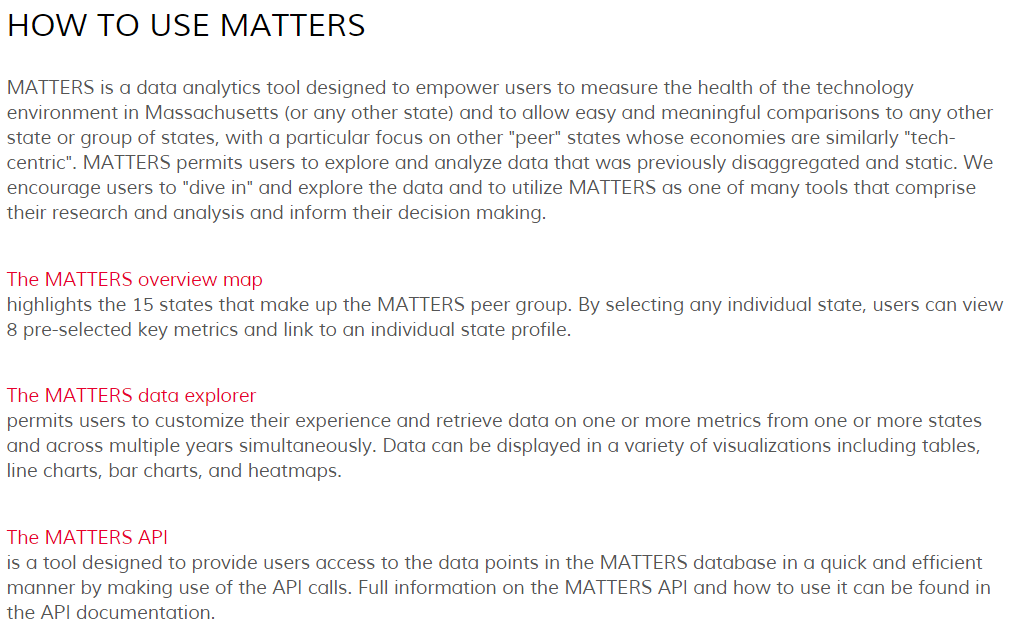
\includegraphics[width=0.75\textwidth]{images/howto.png}}
				\caption{Initial location of the API Documentation link}
				\label{fig:how}
			\end{figure}
		
	\section{Changes made}

		As a result of the user ratings, comments and our observations made while completing 
		the user study tasks, we made a few front end changes to make our features easier 
		to use and easier to find. This included adding a link to the API Documentation in 
		the footer of the site in addition to the link on the "How to use MATTERS" page, as seen 
		in Figure \ref{fig:footer}, and as shown in Figure \ref{fig:edit}, changing the “Create new metric” link on the 
		Data Explorer page to mention that the link would also allow users to edit their metric. 
		
			\begin{figure}[t]
				\centering
					\fbox{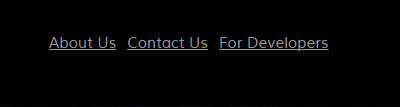
\includegraphics[width=0.75\textwidth]{images/footer.png}}
					\caption{Footer}
					\label{fig:footer}
			\end{figure}
			
			\begin{figure}[t]
				\centering
					\fbox{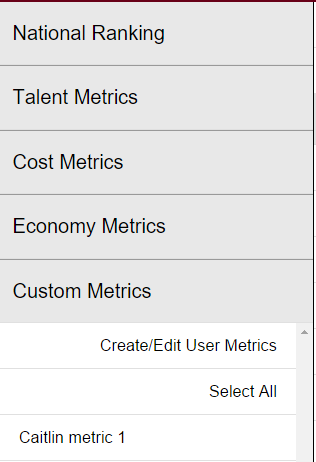
\includegraphics[width=0.5\textwidth]{images/edit.png}}
					\caption{Data Explorer sidebar with edit link}
					\label{fig:edit}
			\end{figure}
			
		These changes led to the final design of the front end of the Metric Builder 
		and API Documentation which can be seen in the figures below. Figures \ref{fig:mb} and \ref{fig:inuse} show the Metric Builder page when a user first visits 
		the page and after a user has selected and assigned weights to some of the metrics from the Metric Selection column of the sidebar. Once the user has decided to save their metric formula, 
		if they choose to go back and edit any part of it, the "Save" button will be replaced by an "Update" button and options are added to "Cancel" any changes or remove the custom metric completely. 
		These additional options can all be seen in Figure \ref{fig:save}. Finally, there were no changes that needed to made to the API Documentation itself as a result of the user testing. 
		Figure \ref{fig:docs}, shows the API Documentation page as it appears when a user first navigate to the page from either the footer or the "How To Use MATTERS" page.

			\begin{figure}[t]
				\centering
					\fbox{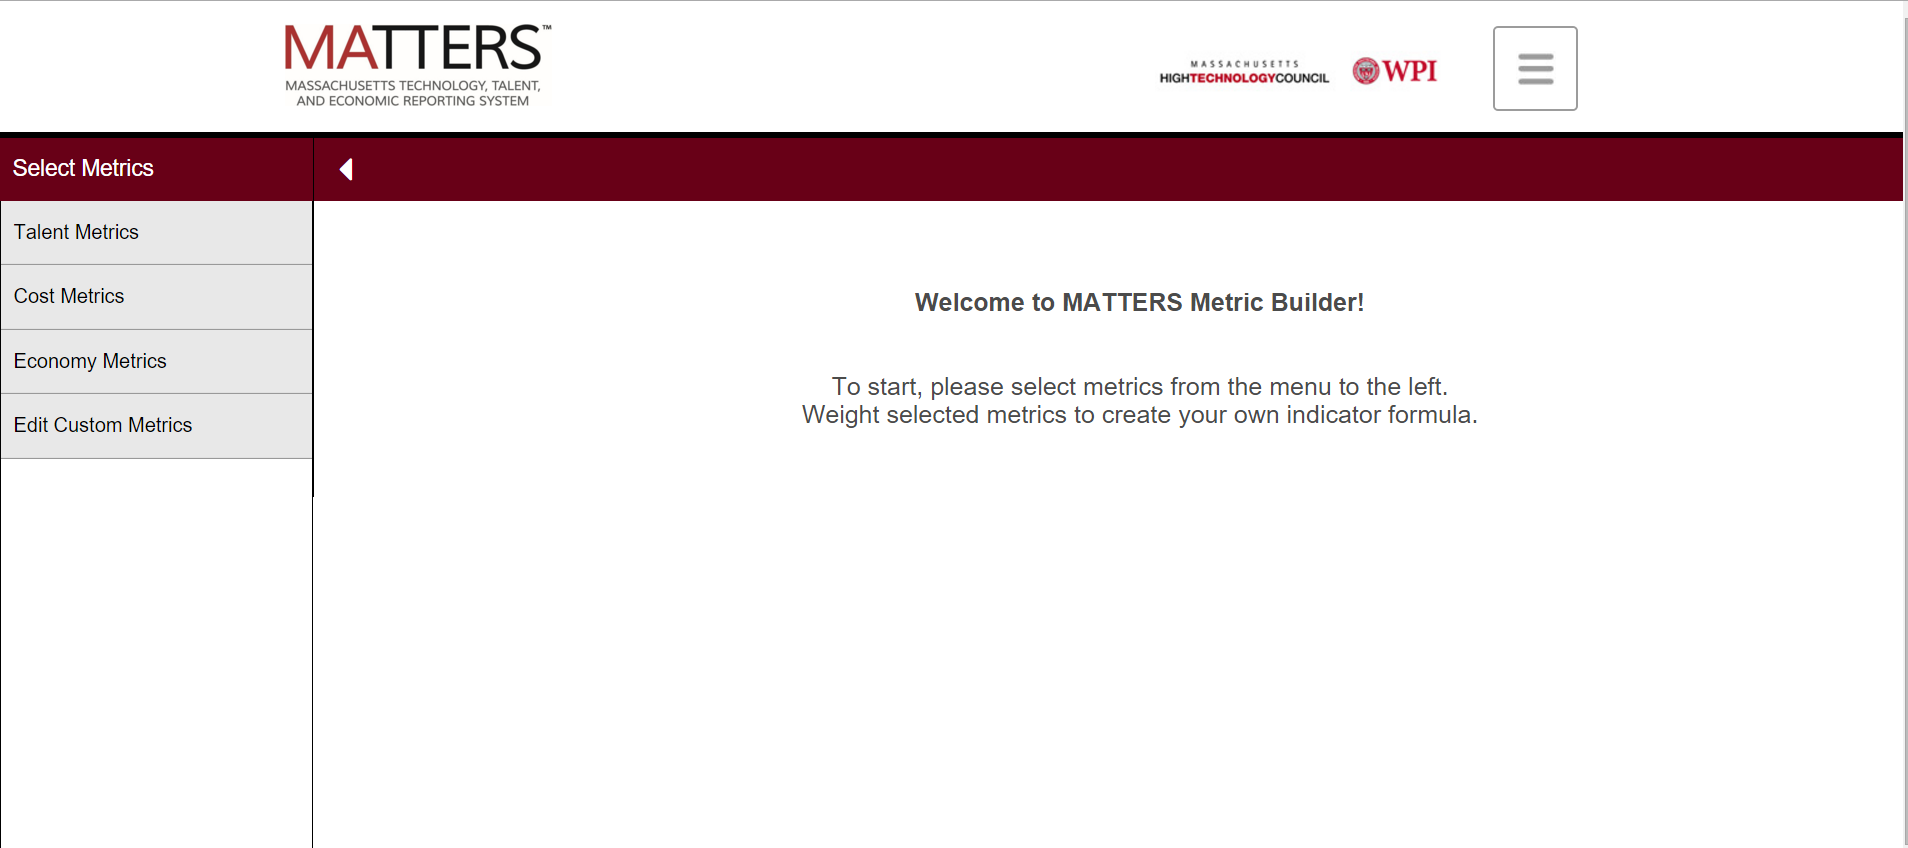
\includegraphics[width=0.75\textwidth]{images/mb.png}}
					\caption{Metric Builder}
					\label{fig:mb}
			\end{figure}
			
			\begin{figure}[t]
				\centering
					\fbox{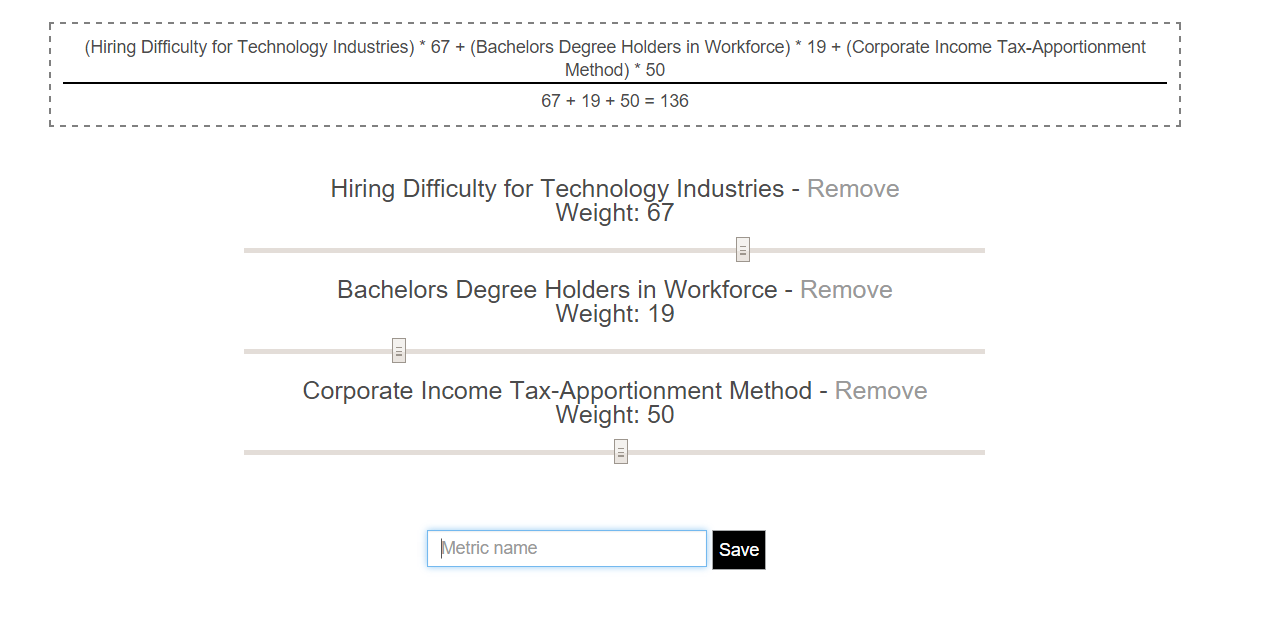
\includegraphics[width=0.75\textwidth]{images/using.png}}
					\caption{Metric Builder's canvas}
					\label{fig:inuse}
			\end{figure}
			
			\begin{figure}[t]
				\centering
					\fbox{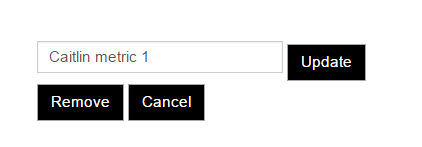
\includegraphics[width=0.75\textwidth]{images/saved.png}}
					\caption{"Save" menu}
					\label{fig:save}
			\end{figure}
			
			\begin{figure}[t]
				\centering
					\fbox{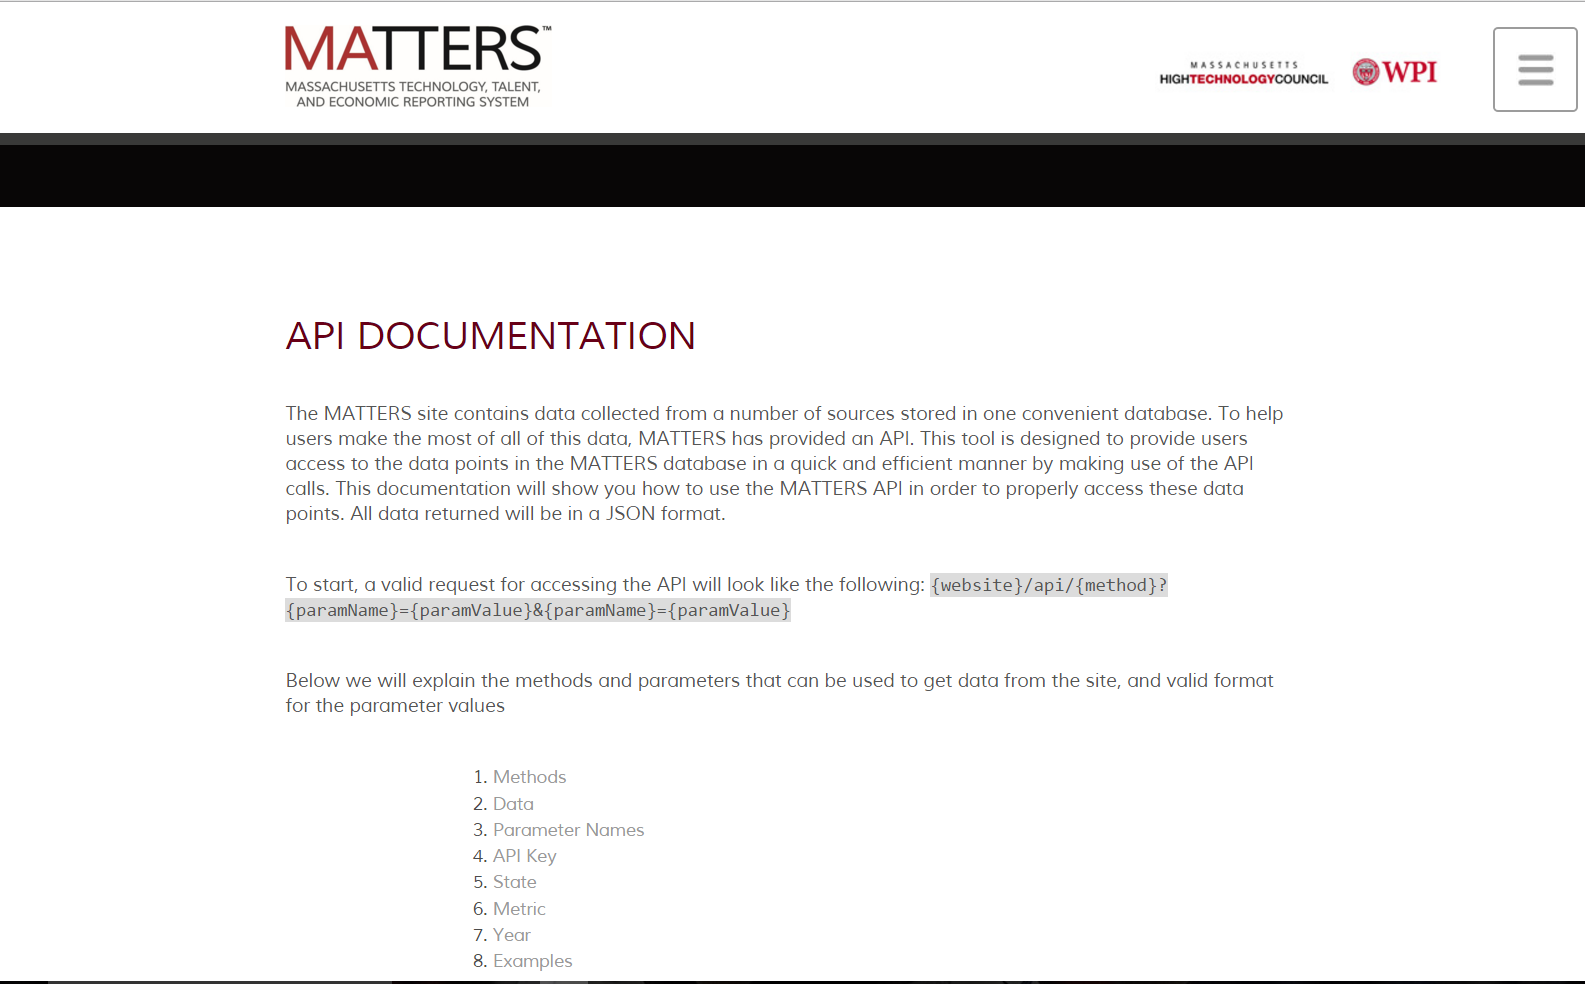
\includegraphics[width=0.75\textwidth]{images/api.png}}
					\caption{API Documentation page}
					\label{fig:docs}
			\end{figure}
    
    \chapter{Conclusion}

	In this project we have built two important services for the MATTERS site that enhances its capabilities and thus value. The API 
	provides a way for other computer-based systems to work with the MATTERS 
	system. Specifically, it is now possible to query MATTERS data directly via a software program 
	bypassing the presentation layer. This is extremely useful because it now empowers MATTERS' data warehouse to serve as a portal for important aggregated economic data.
	The other feature is the Metric Builder. 
	This service allows users to create their own personalized metrics based on 
	the existing metrics. This is useful as before users could only visualize the data of preexisting metrics, and MHTC and other users can now easily use their own personal idicators. 
	Users are able to work with their custom metrics seamlessly 
	in the Data Explorer as if they were just regular ones.  

	\section{Recommendations}
		
		Recommendations for other teams, either MQP or other teams, working on improving the MATTERS system in the future are as follows:
		
		\begin{itemize}
			\item MATTERS system
				\begin{enumerate}
					\item
						Let users define more complex equations for their user metrics.
						User should not be limited by simple weighted average formula.
					\item
						Let users suggest their own data or data sources. Right now 
						MATTERS' administrators and data management team are working on
						adding data. By involving users in this process MATTERS may have 
						more complete, accurate and up-to-date data.
					\item
						Role management. Right now the system supports regular users and API users. 
						Each user metric must have one and only one author. It would be useful 
						to merge these two user entities and introduce shared user metrics that are 
						not bound to specific users.
				\end{enumerate}
			\item Software development
				\begin{enumerate}
					\item
						Refactor the client side and server side code. Since the system 
						has been developed by a number of teams with different design 
						patterns and approaches, there is a significant technical debt. 
						It might be worth spending some time rewriting parts of the system 
						according to the latest coding and technical standards.
					\item
						Documentation. Right now there is a steep learning curve for new 
						developers who start working on the project. Good documentation would 
						dramatically decrease the time it takes for developers to start working 
						on the project.
				\end{enumerate}
		\end{itemize}


    \bibliographystyle{unsrt}
    \bibliography{bibliography/references}

\end{document}